\begin{center}
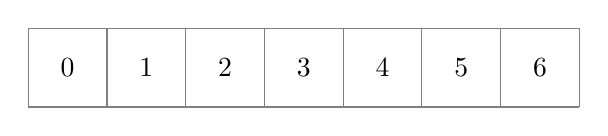
\begin{tikzpicture}
	\draw[step=1cm,gray] (0,0) grid (7, 1);
	\node at (0.5, 0.5) {0};
	\node at (1.5, 0.5) {1};
	\node at (2.5, 0.5) {2};
	\node at (3.5, 0.5) {3};
	\node at (4.5, 0.5) {4};
	\node at (5.5, 0.5) {5};
	\node at (6.5, 0.5) {6};
\end{tikzpicture}
\par\noindent {\scriptsize Figura 2: Representação gráfica do ambiente do agente}
\end{center}